% Chapter Template

\chapter{Results} % Main chapter title
%choose two or three projects, check report

\label{Chapter4}

\section{Statistics}

\subsection{Description}
As described in the previous Chapter, the "Statistics" project is an external feature in Agent's dashboard that reveals total rides and Gross Merchandise Volume (GMV) gained from BeatHotel service. More specifically, there were added charts in the BeatHotel's web application that present data based on what KPI, resolution, and period of time will be chosen by Agents. The term KPI is referred to either Completed Rides, or GMV, or Cancelled Rides, while term "resolution" applies to yearly, monthly, weekly, daily or even hourly analyses of data. In the chart, it is also compared to the given period's data with the previous week's or year's data. \par

\subsection{Deliverables}
This project had three main deliverables so as to be completed, npm package creation, customized Statistics, and General Statistics. \par

\subsubsection{Npm Package}
The first deliverable is the creation of an npm package as described in Appendix 8.1, showing the project's ReadME.md file. The package can be used in both front and back-end applications, and it returns one function and two objects, which are the KPI and resolutions object. \par 
As regards the function, it receives five arguments. The first argument given, named "statsObject", is an object of the gathered data saved in firebase, BeatHotel's real-time database. The other two arguments are the starting and ending timestamps of the desirable data's period of time, while the remain ones determine the KPI and resolution of the received data. The purpose of this function is to return an object that format data received from the database based on its parameters. \par
For privacy reasons, it is not possible to cite the code written. However, it can be mentioned that code was developed in ES6 JavaScript, consists of 303 lines of code, both comments and pure code, and it includes eight functions in total. Moreover, there were created unit tests in Jest and are in total 395 lines examining ten different use cases. Code is using enlist-styling and includes babel in its webpack configuration so as to be used in both front-end and back end projects if it is needed. \par

\subsubsection{Customized Statistics \& Dashboard KPIs}
After the npm package creation, I had to present the data on the Agent's web application. So, I created and added on tab Dashboard of BeatHotel web page, two customized charts and two more cards that reveal this week's Rides and GMV, as shown in the red square of figure 4.1.   \par
Regarding the customized charts shown, there is one for showing rides per day and one for GMV. Both charts have two lines. The blue line is created based on the current week's data, while the gray one by last week's. Generally, their purpose is to compare this and last week's rides and GMV. For this reason, a week on week (WoW) percentage is shown at the top left of the charts which is referred to this comparison. Percentage representation is also changing color, from green to red, and arrow's direction, from up to down, if needed. Last but not least, we need to mention that charts are updated on refresh, so the timer down left displays when the data were lastly updated. \par 
Additionally, I was requested to add two more cards, one for Rides and one for GMV KPI. These cards are referred to data gathered from the beginning of the current week (Monday 00:00) until the day and time Agent is using the dashboard. Furthermore, they demonstrate how many Rides or GMV BeatHotel service had the last seven days passed. One last detail about cards is that the color of icons, in the picture shown as green, is changing to either green, orange or red depending on the WoW percentage described earlier. \par

\begin{figure}[H]
	\begin{center}
		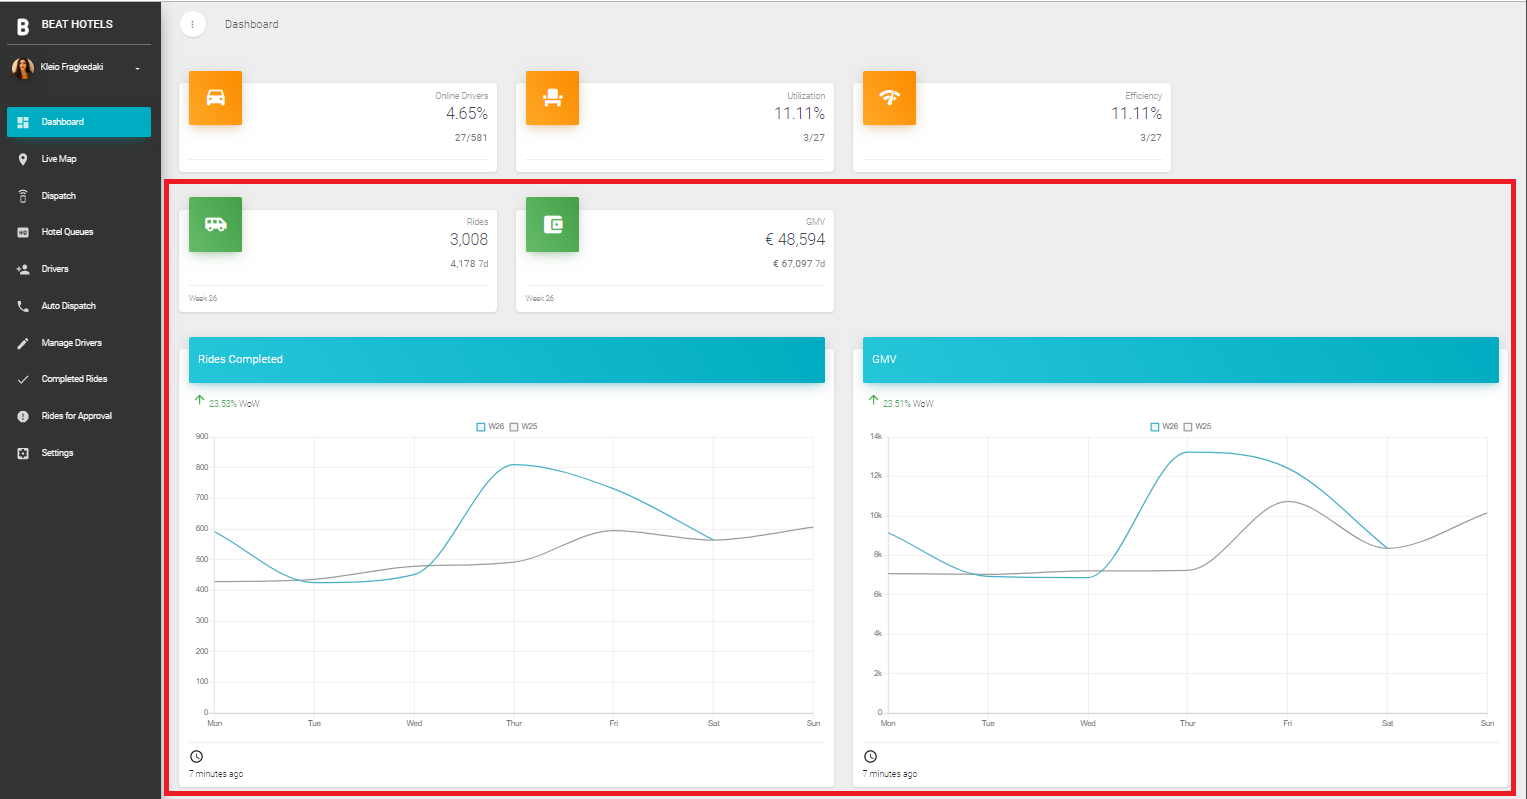
\includegraphics[scale=0.45]{images/my_projects/Statistics/feature-dashboard-statistics.png}
	\end{center}
	\caption{Customized Statistics}
\end{figure}

In technical detail, there were added 610 and removed 62 lines of code in total 12 files. More specifically, four main components were created, that is Timer.jsx, RideChart.jsx and DashboardInfo.jsx, DashboardKPIContainer.jsx. The last one was created for abstracting already existing Card's Component and reuse it for developing the new ones in order not to repeat a similar code. \par

\subsubsection{General Satistics}

One more aspect of charts is the "General Statistics" where it can be chosen for which KPI or dates you want to receive data. In this sense, there is a dropdown where you can choose the KPI, either GMV, Completed or Canceled Rides, and two inputs one for the starting and one for the ending date of the data displayed. "General Statistics" is basically the same charts as the customized ones, but with the preferred data shown and more functionality into them. \par
In figure 4.2, it is shown how "General Statistics" look like. However, we need to mention that this project was never completed and fulfilled with a Pull Request on GitHub(PR) because of other priorities. This is the only project that is not currently in production. \par


\begin{figure}[H]
	\begin{center}
		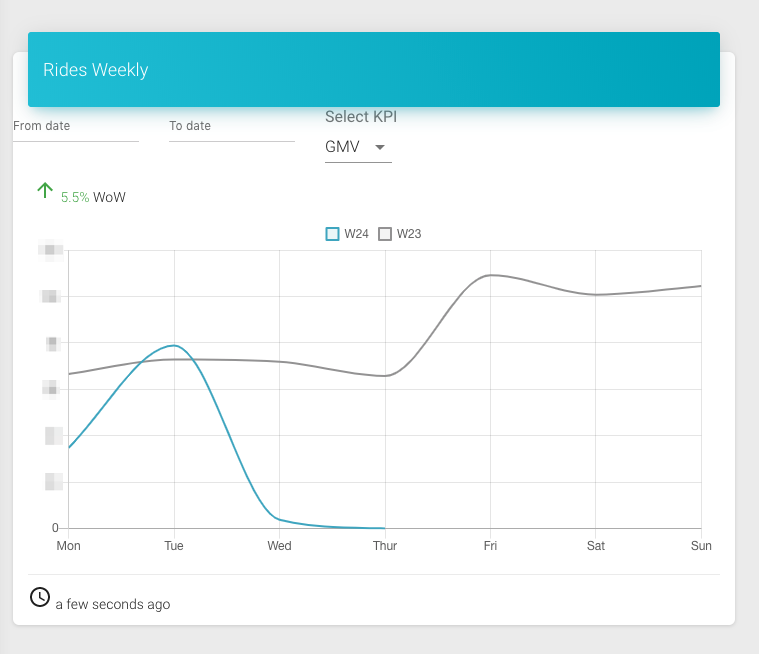
\includegraphics[scale=0.3]{images/my_projects/Statistics/General_Statistics.png}
	\end{center}
	\caption{General Statistics Overview}
\end{figure}


\subsection{Best Practices \& Main Tools/Methods Used}

Several tools and practices taught in quite a few courses in Management Science and Technology Department have been used to fulfilling this project's needs. More specifically, JavaScript and other web development tools taught during the Information Systems Implementation \& Architecture course of the 5th semester, and Internet \& Cloud Application Development course of the 7th semester was the most useful knowledge gained. Furthermore, the GitHub usage required for the project was given from the 6th semester's course in Software Engineering in Practice. \par

\subsection{Total Hours spend on the Project}

This project consists of both back and front end implementations, and it has to be mentioned that "Statistics" was one of the first projects in JavaScript and the first one in ReactJS that I had to complete. So, the total working hours spend on the Project were about to 72, with other features and bug fixes running at the same time as shown on Gantt Chart below. \par

\subsection{Delays on Initial Schedule}

This project is separated into three main parts and each part had its own schedule. The first part referred started on April 11 and ended on April 20, while the second on April 24 and ended on April 27. The last part of "General Statistics" was included in the second part, but it was never completed, since it was not defined how the design and the whole logic should be, and it stopped being a priority. \par

Finally, my PR on GitHub about this feature was merged on May 22, while on May 24 it was online on BeatHotel Agent Dashboard.

\begin{figure}[H]
	\begin{center}
		
\includegraphics[scale=0.85]{images/my_projects/Statistics/feature-dashboard-statistics-PR.png}
	\end{center}
	\caption{Approved Pull Request}
\end{figure}

\subsection{Problems occurred}

During the implementation of the project, there were some problems regarding both procedural and coding issues. First of all, I had to get access to Beat's npm account so as to upload stats package. For this reason, there were procedural delays for getting access and eventually upload the created package. As regards coding issues, creating an npm package for both client and server side is not that easy. You need to get to know babel so as the ES6 code to be transpiled in ES5, which is the language browser understands. Finally, jest created for the package's unit testing was not executed when the project started using with babel. \par

\subsection{Estimation of Project's impact in the company}

The results of this specific project are important for Beat's Agents. The charts displayed on the dashboard are providing information showing how rides and GMV are on a weekly basis, and how the current week is compared to the previous one. This information is giving a sense of how good business is going and if it is needed something to be done immediately.

\section{Landing page for mpaineis-vgaineis}

\subsection{Description}

Landing page project is a web site for \href{mpaineis-vgaineis.gr}{mpaineis-vgaineis} competition which is referred to Beat users. Regarding the competition, GR Marketing team launched an event in which every week one participant would win a trip abroad. The competition lasted four weeks in total, and every week there was a different destination starting from the 10th of June. My role in this competition was to create a landing page through which every possible user could declare interest in the event, and in this way, to win a trip for two people. \par

In much more detail, the landing page was developed in ReactJS. There were designs for the web page provided via Zeplin, a program exporting designs from Adobe XD, Photoshop CC, and other projects to CSS code. Thus, it was used CSS, and the beat-ui theme for matching the designs in each possible device, as described in Appendix 8.2. It is needed to mention that the landing page was based on another project, a fact that occurred issues and unused components. In total, I added more than 9,000 pure lines of code, deleted more than 14,000 lines. More specifically, about to 10 jsx components, 4 .js files, 15 .css files were created, while 35 other files were deleted. In general, the landing page had seven main components, the Header, Video Display, Event's description, Application form, Download app, Social media, Footer, Term and Pop-up Configuration, as figures 4.4, 4.5 and 4.6 display. \par

As regards the functionality of the page, Video display has one clickable button that leads to a video created for the announcement of the competition in social media. Additionally, the Application form component includes two inputs, one for email and another for phone, while there is also a checkbox for the participant's agreement with the terms and a button for submitting the form. After clicking the submit button, there are two main use cases either the user sees a pop-up like the one shown in picture 4.6(A) for submit confirmation or sees check-box, email or/and phone input to have red borders. This is happening in case the previously mentioned fields are not correctly completed or not completed at all.  In the first case where the confirmation pop-up is displayed to the user, a callable function is called from the server side that validates data and then writes to Firebase and BigQuery participant's email and phone. Due to both front and back are checking the data typed in the form, there is also one more case where the validation passes from the front and not from the back-end and a pop up is appeared saying "Oops Something went wrong, try again!". \par

\begin{figure}[H]
	\centering
	\subfloat[Header \& Video Display]{{\includegraphics[scale=0.07]{images/my_projects/landing_page/header.png} }}%
	\qquad
	\subfloat[Description \& Form]{{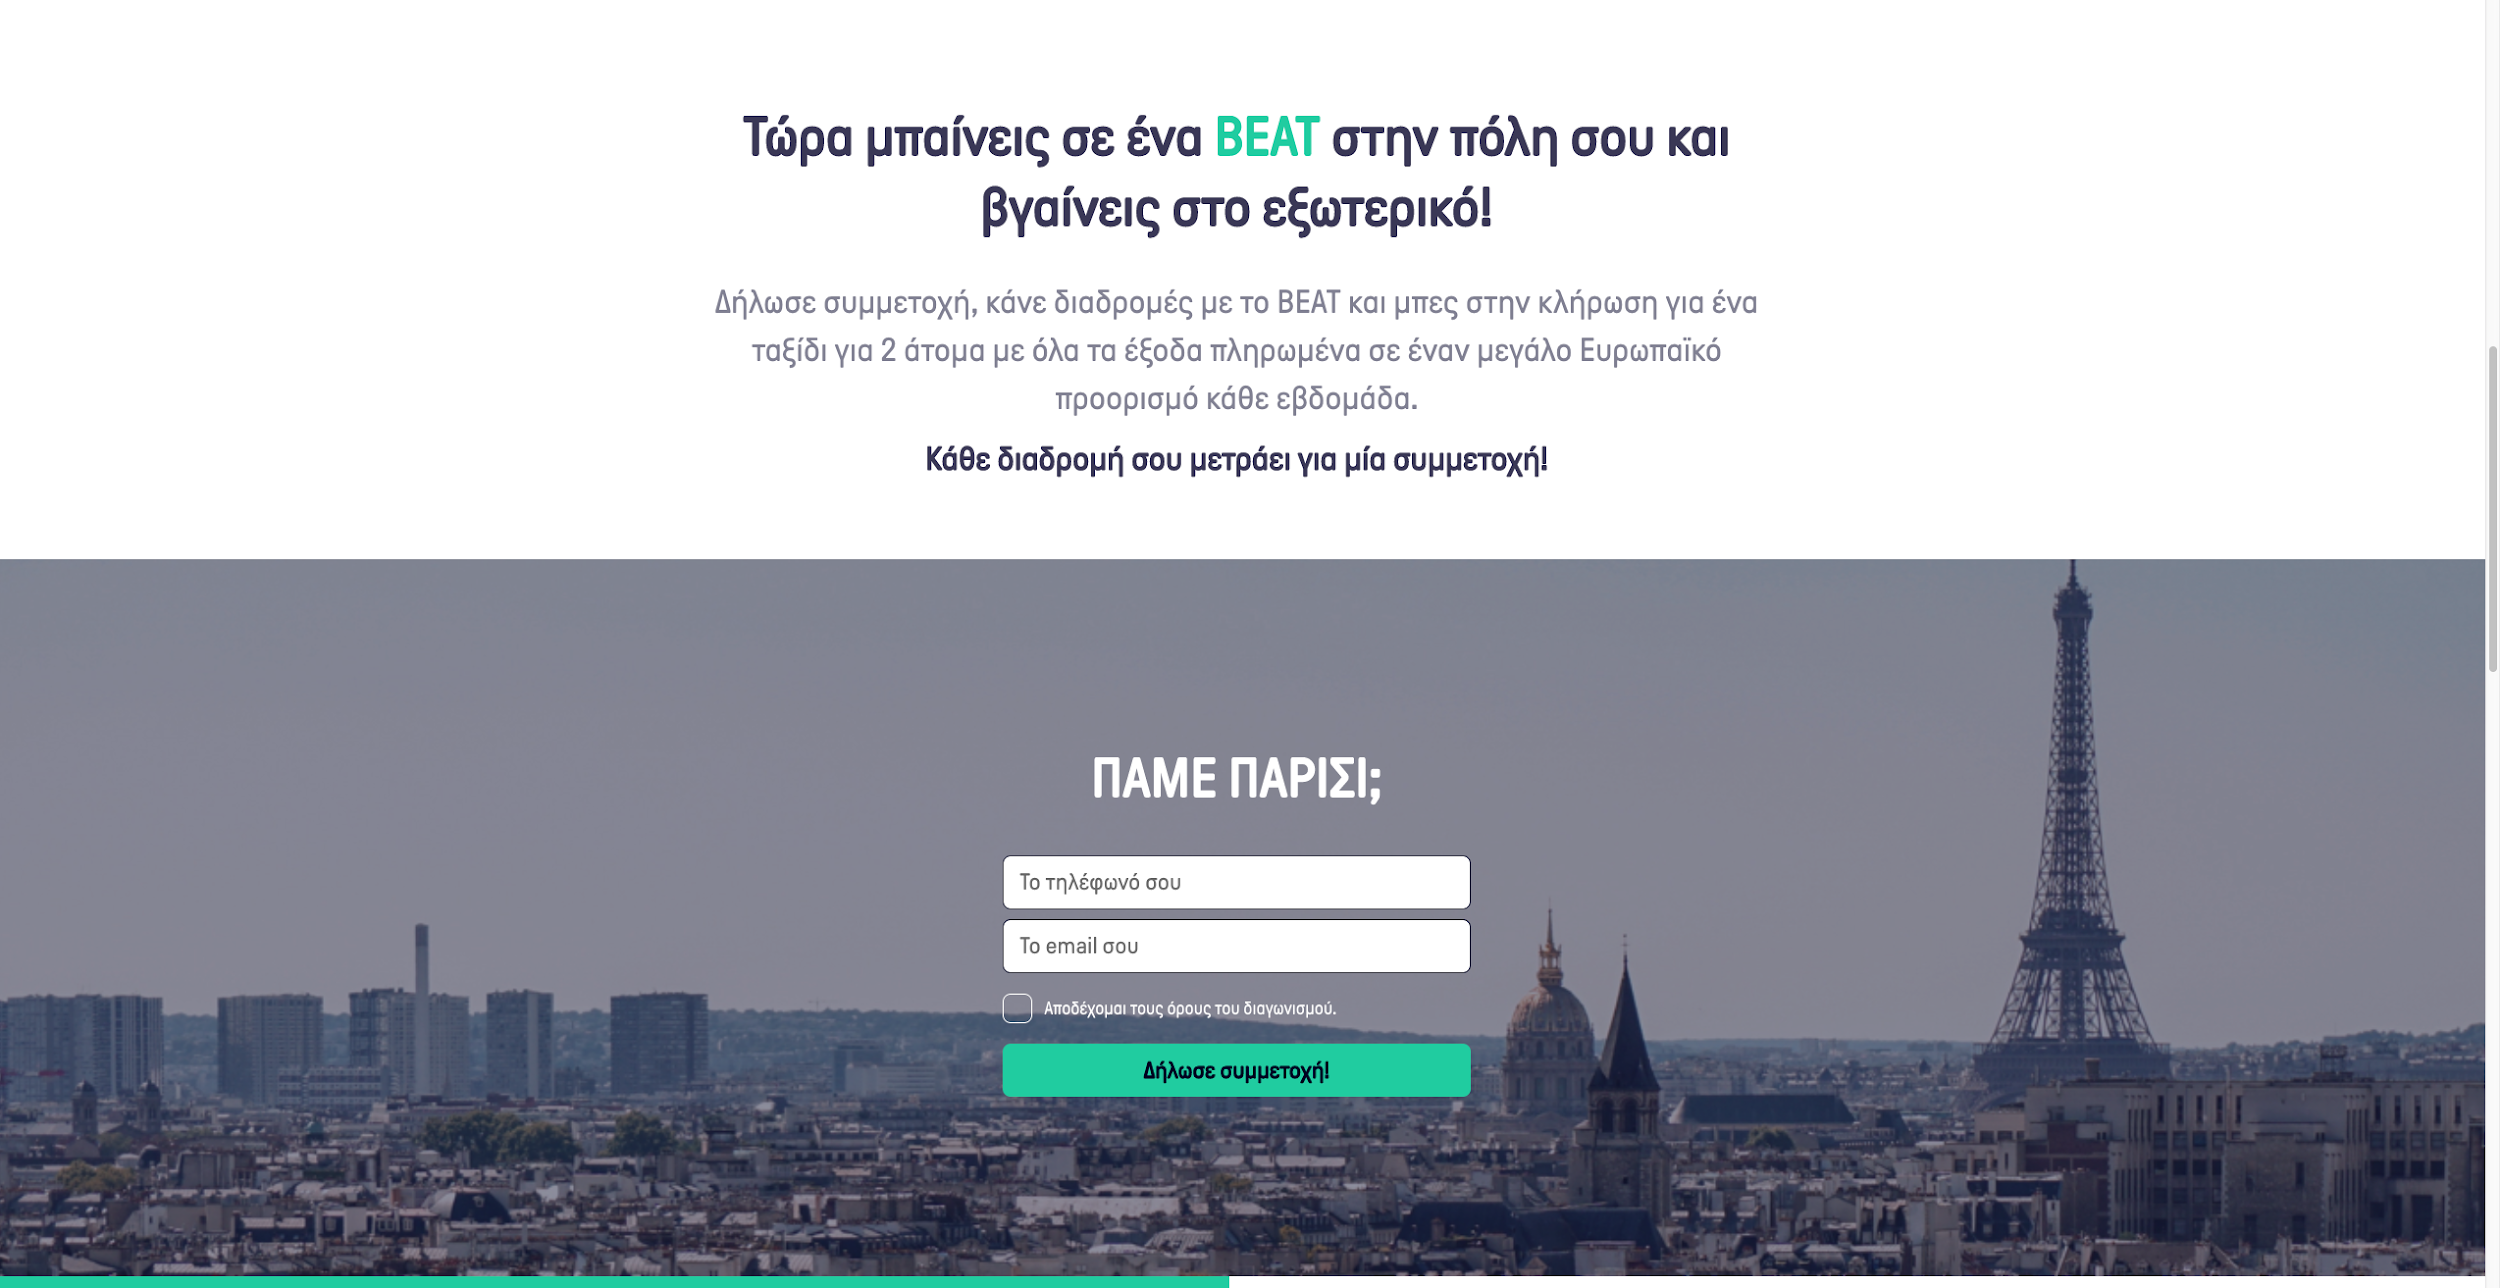
\includegraphics[scale=0.07]{images/my_projects/landing_page/form.png} }}%
	\caption{
		Landing Page for Competition mpaineis-vgaineis
		\\
		\textbf{Online: } \url{https://mpaineis-vgaineis.gr/}
	}
	\label{fig:example}
\end{figure}

In figure 4.5 (A), Download App component is divided into two part's that in case of mobile display they are one upon the other. The second part has a button that redirects user to either PLay Store or Apple Store of the Beat App depending on the user's device, as found in \href{https://l.facebook.com/l.php?u=https\%3A\%2F\%2Fstackoverflow.com\%2Fquestions\%2F38241480\%2Fdetect-macos-ios-windows-android-and-linux-os-with-js\%3Ffbclid\%3DIwAR3uoMdkjVLP4sYZwZYNdWZvnU6ZENl_ydezZUYBDrDXcAuMZ7TKWHR1_rs\&h=AT106TjLH1q4m5FXvHR8F5OLOxARMZ07jIj0a5JeCLWiptBV09H1oPWquvUAykdDj_jEyBSwHwd_ELvKjCUjKGg5FkErIz0jFkG_QK8vfVCOOJfxAjxHPj11YPc4-Jf8JFgCjA}{Stackoverflow}. Last but not least, in the bottom of web page, there is the Social Media component that includes three buttons opening a new tap to Beat's social media, while the Footer component contains competition's term, which is the pop-up shown in picture 4.5 (B). \par

\begin{figure}[H]
	\centering
	\subfloat[Download App]{{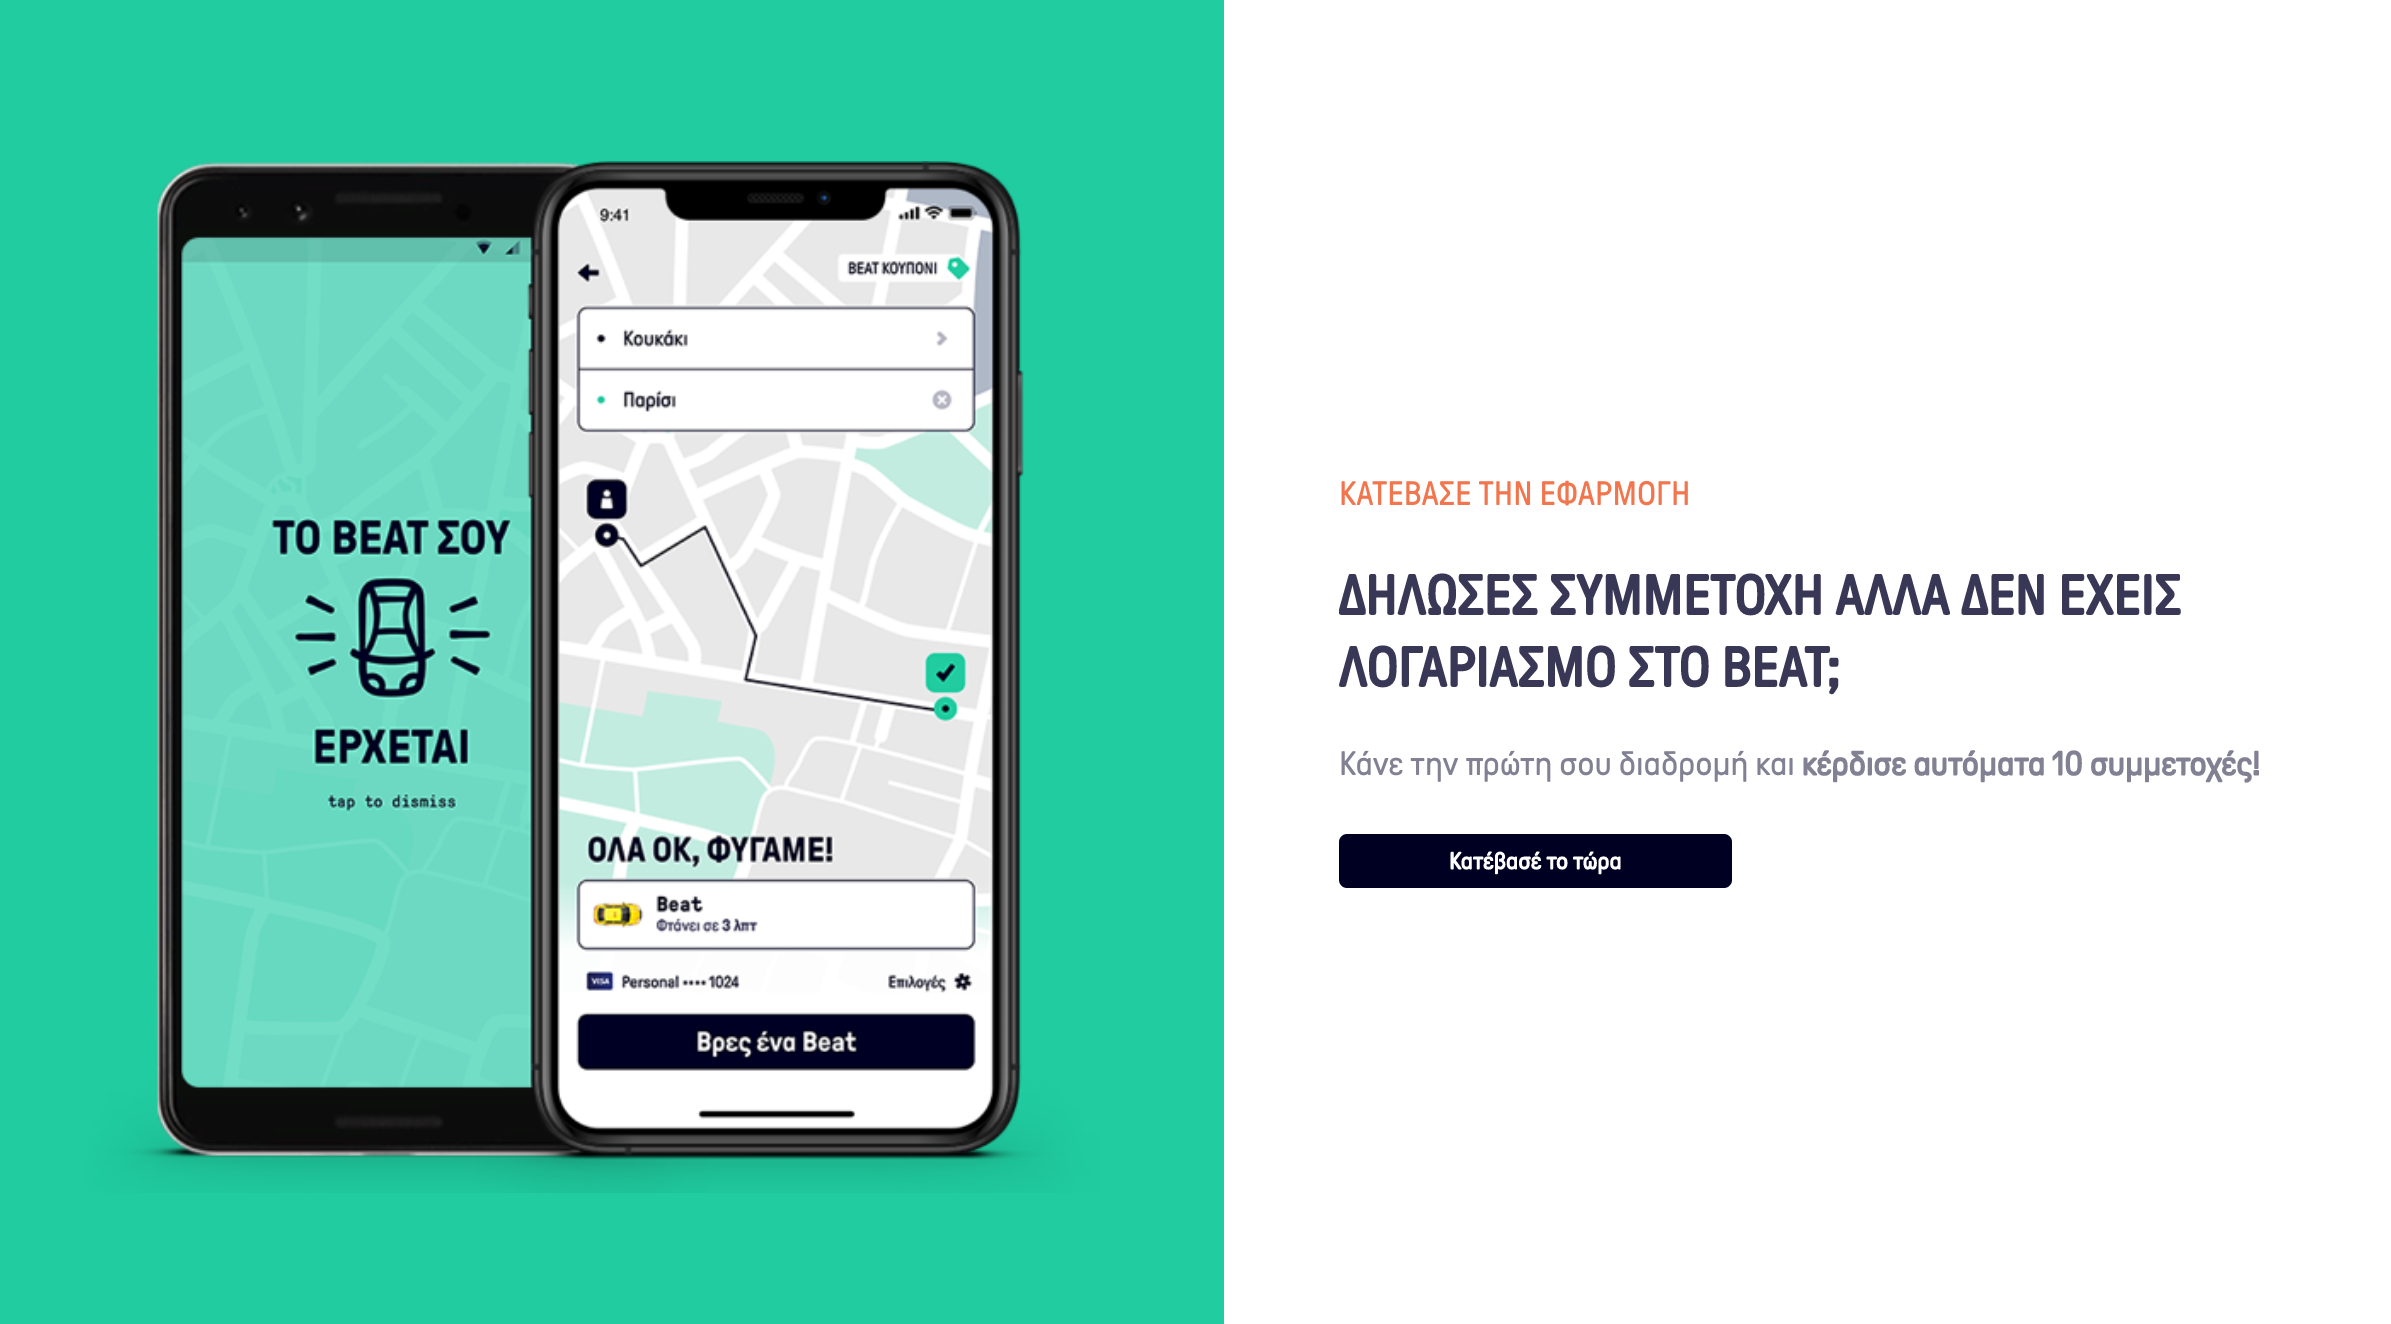
\includegraphics[scale=0.07]{images/my_projects/landing_page/app.png} }}%
	\qquad
	\subfloat[Social Media \& Footer]{{
\includegraphics[scale=0.07]{images/my_projects/landing_page/footer.png} }}%
	\caption{
		Landing Page for Competition mpaineis-vgaineis
		\\
		\textbf{Online: } \url{https://mpaineis-vgaineis.gr/}
	}
	\label{fig:example}
\end{figure}

Following, there are the two pop-ups one for confirmation when submitting the form and one for terms display. The whole project uses a specific manually added font-family called "Pressura", which is Beat's special characters. \par

\begin{figure}[H]
	\centering
	\subfloat[PopUp Confirmation]{{
\includegraphics[scale=0.3]{images/my_projects/landing_page/popup-confirmation.png} }}%
	\qquad
	\subfloat[PopUp of Terms]{{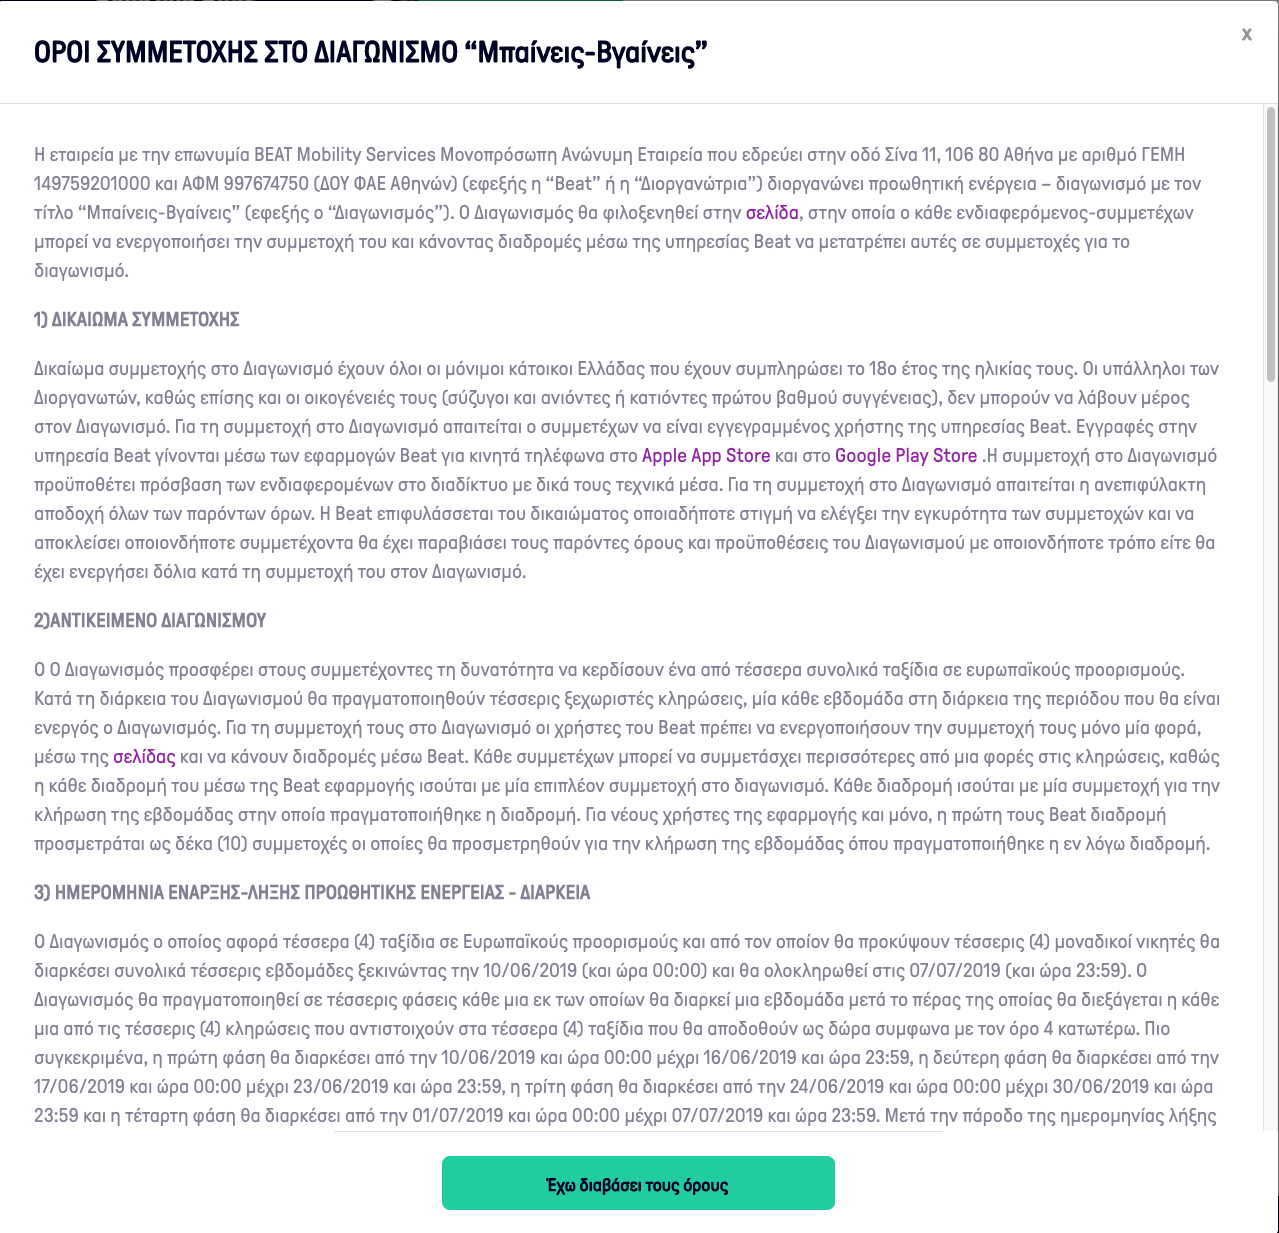
\includegraphics[scale=0.13]{images/my_projects/landing_page/limits.png} }}%
	\caption{
		Landing Page PopUps for Competition mpaineis-vgaineis
		\\
		\textbf{Online: } \url{https://mpaineis-vgaineis.gr/}
	}
	\label{fig:example}
\end{figure}

\subsection{Best Practices \& Main Tools/Methods Used}

To complete this project, I used some practices and methods taught during my studies in Management Science and Technology Department. More specifically, the Information Systems Implementation \& Architecture course of the 5th semester gave me the knowledge of JavaScript, CSS and generally theme libraries. Firebase usage, creating reusable components and the way to deploy my app was learned via Internet \& Cloud Application Development course of the 7th semester. Finally, the course of the 6th Semester named Secure Software Development provided useful information about how the network works and how to build a secure application. \par

\subsection{Total Hours spend on the Project}

The landing page of mpaineis-vgaineis is the biggest project I was part of. It lasted approximately one week and the total working hours spend on this project was about forty. \par

\subsection{Delays on Initial Schedule}

This project was assigned to me on the 30th of May and it had to be hand on the 8th of June since the event was about to start on Monday the 10th of June. There were some delays during the project regarding my access to beat-ui theme and because of Marketing and designs postpones. Referring to the last applied reason, videos, photos, and terms needed for the landing page were sent the same day of my deadline, a fact that caused problems. \par

The landing page is visible to every user until July 7th at \url{mpaineis-vgaineis.gr}.

\subsection{Problems occurred}

There occurred three main problems during the implementation of this project. First of all, it was based on the top of a totally different project, which was not even upgraded and had a lot of extra components that had to be deleted. Developing a project that is based on another one is both inflexible and time-consuming because of upgrading all libraries. Another core problem was that designs were changing and pictures, video and term's conditions were not given until one working day before the competition. Last but not least, displaying the given designs in each possible device was also time-consuming and not that easily performed. \par

\subsection{Estimation of Project's impact on the company}

The completion of this project was one of the main parts of the competition launched. Thus, its results had a large impact on Marketing's event, and more specifically in people's eyes regarding Beat. \par

\section{Input Different Pick-Up Location}

\subsection{Description}

BeatHotel is generally a B2B service that firstly aimed to fulfill the needs of hotels for a virtual cub queue. For this reason, the service's dashboards, which is the only way Beat's Agents or Hotels to request for a taxi, used to have only one pick-up location, the Hotel asked for the taxi. However, as the business grows, travel agents, that started to be part of the system, and some hotels needed to complete rides with different than Hotel's pick up location. Thus, I needed to refactor the Dispatch page, change modal so as to be responsive and add an input for typing any possible different pick-up location. \par

Figure 4.7 reveals the differences between the old (A) and the new (B) dispatch page. First of all, I removed the two toggles of POS and Staff and changed the position and appearance of "Request a taxi" button to a circle with just a plus sign. Moreover, I added a hover to each row displayed in the queue of every Hotel, which shows the pick-up location of the ongoing rides. \par

\begin{figure}[H]
	\centering
	\subfloat[Old Dispatch Tab]{{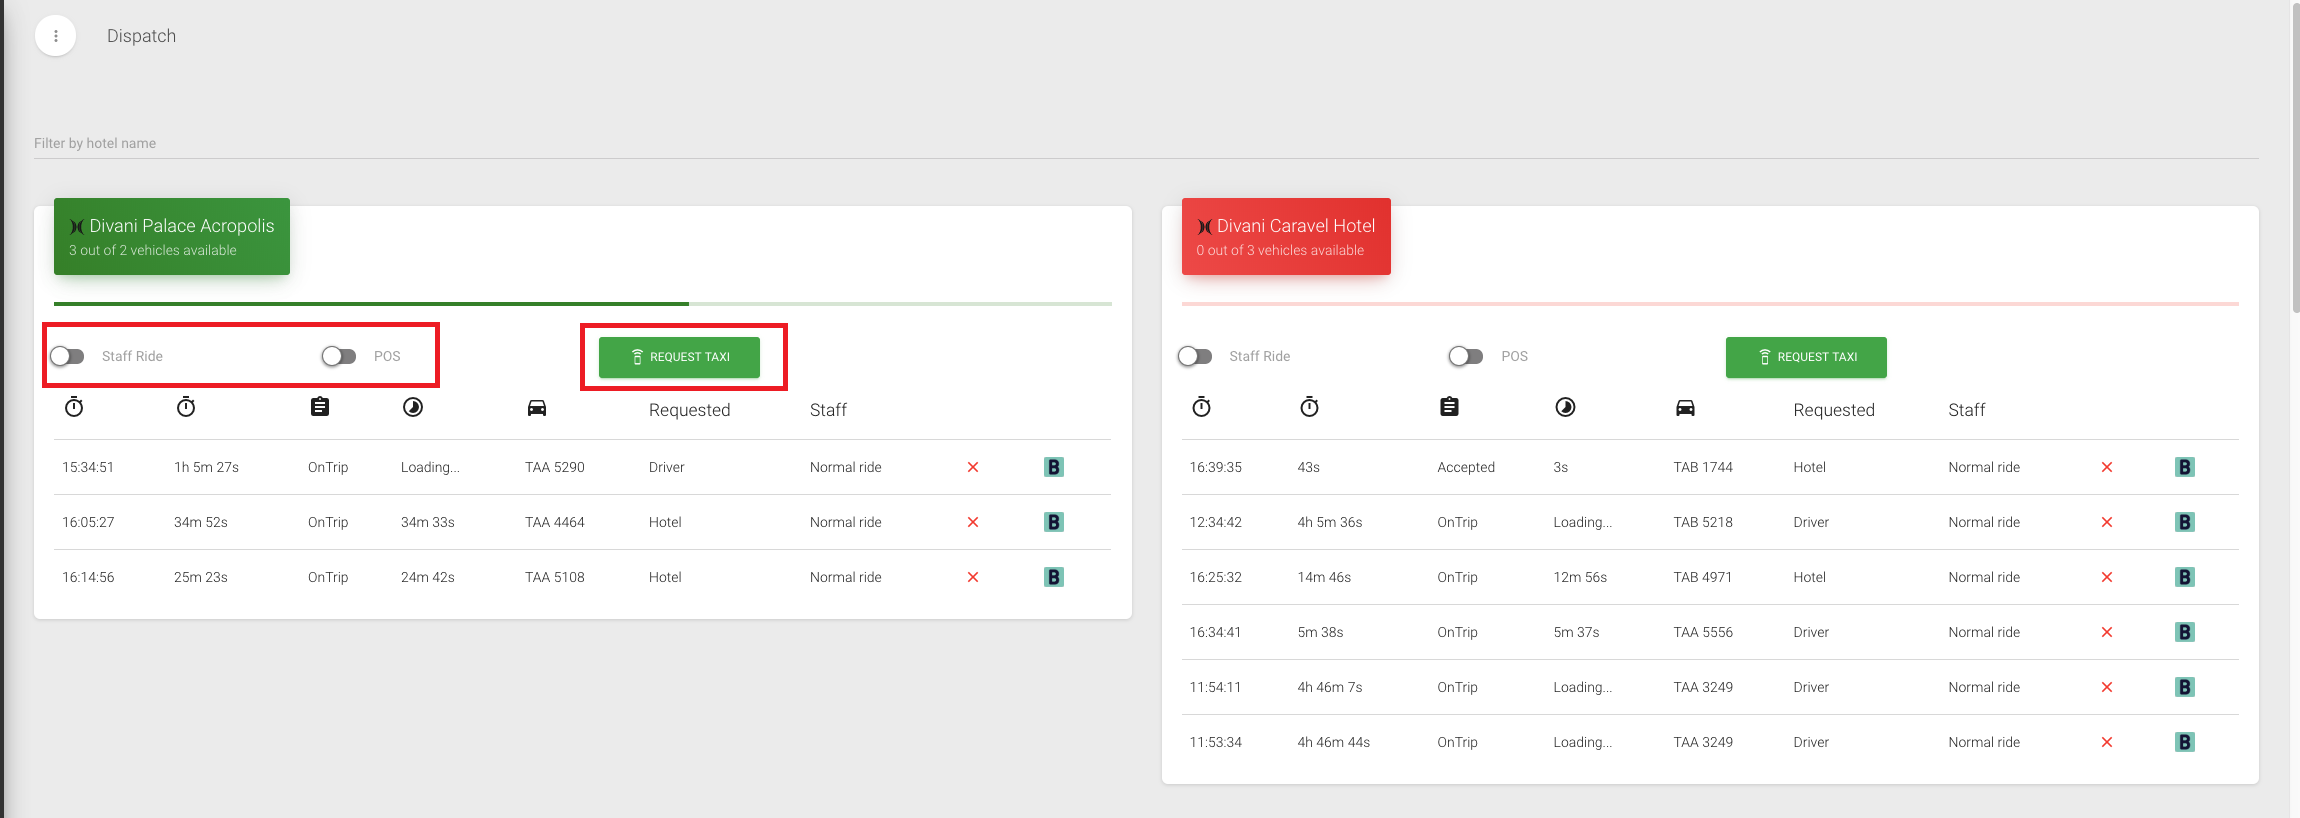
\includegraphics[scale=0.23]{images/my_projects/input/input-location-dashboard-old.png} }}%
	\qquad
	\subfloat[New Dispatch Tab]{{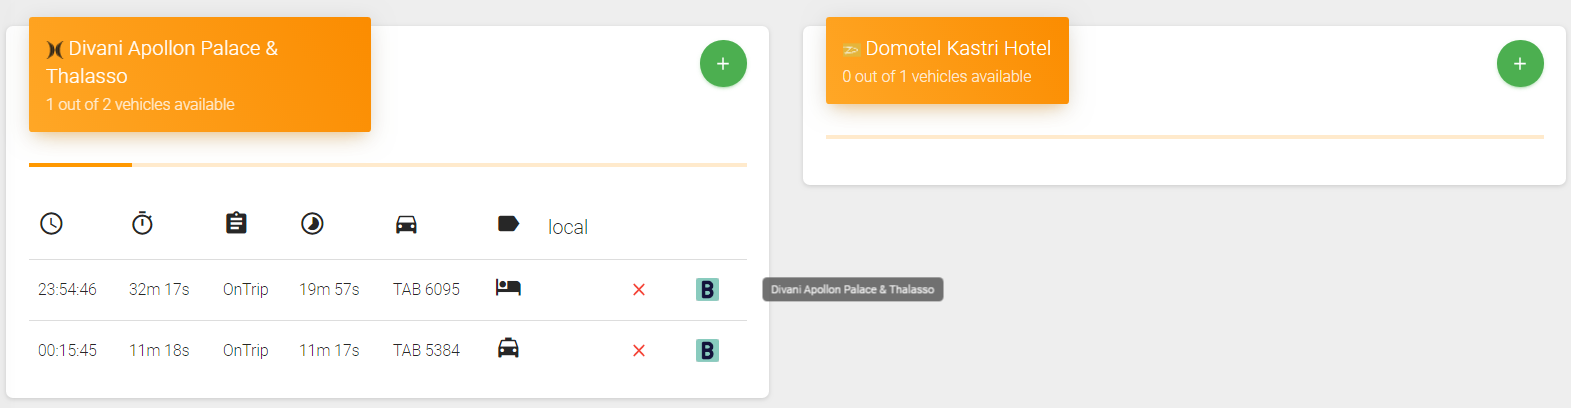
\includegraphics[scale=0.35]{images/my_projects/input/input-location-dashboard-new.png} }}%
	\caption{
		Reconstruct Dispatch Components for requesting a taxi from Agent's Dashboard
	}
	\label{fig:example}
\end{figure}

When the "plus" button is clicked, a pop-up for requesting a taxi appears. This pop-up includes all the possible options that can be activated for the ride, such as Staff Ride, POS, Note to Driver, that were also provided in the previous version. There is an additional option of changing the pick-up location, as shown in picture 4.8 (B) and 4.8(C). By default, the input bar is filled with the selected Hotel or travel agency location, which can be changed by typing the desirable address and picking one of the dropdown options revealed. In this way, latitude and longitude of the pick-up location are changed and send to the driver as soon as the pop-up's Dispatch button is pushed.

\begin{figure}[H]
	\centering
	\subfloat[Previous Version]{{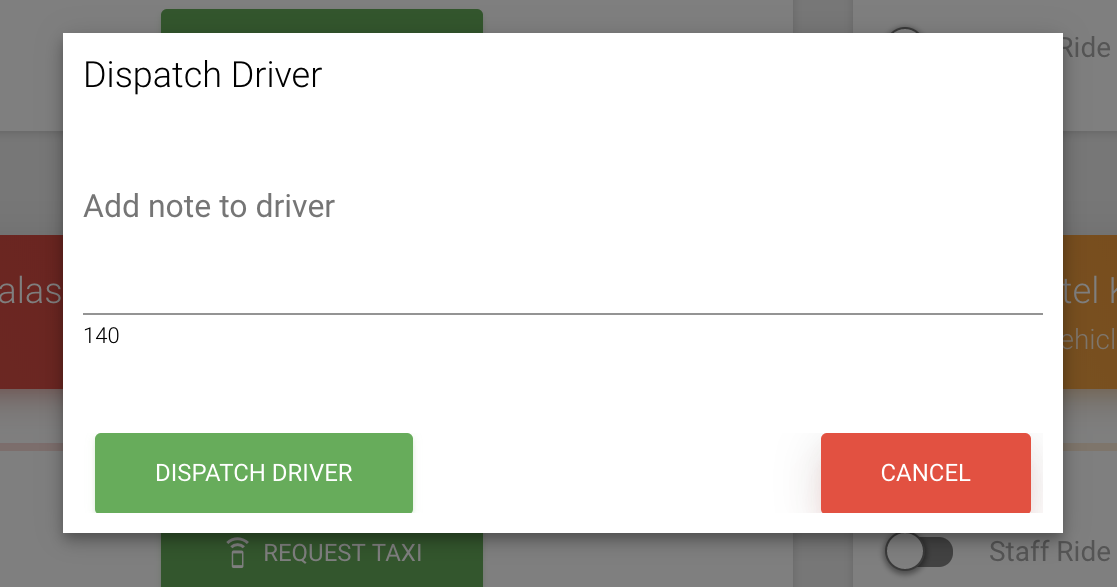
\includegraphics[scale=0.24]{images/my_projects/input/input-location-popup-old.png} }}%
	\qquad
	\subfloat[New Version]{{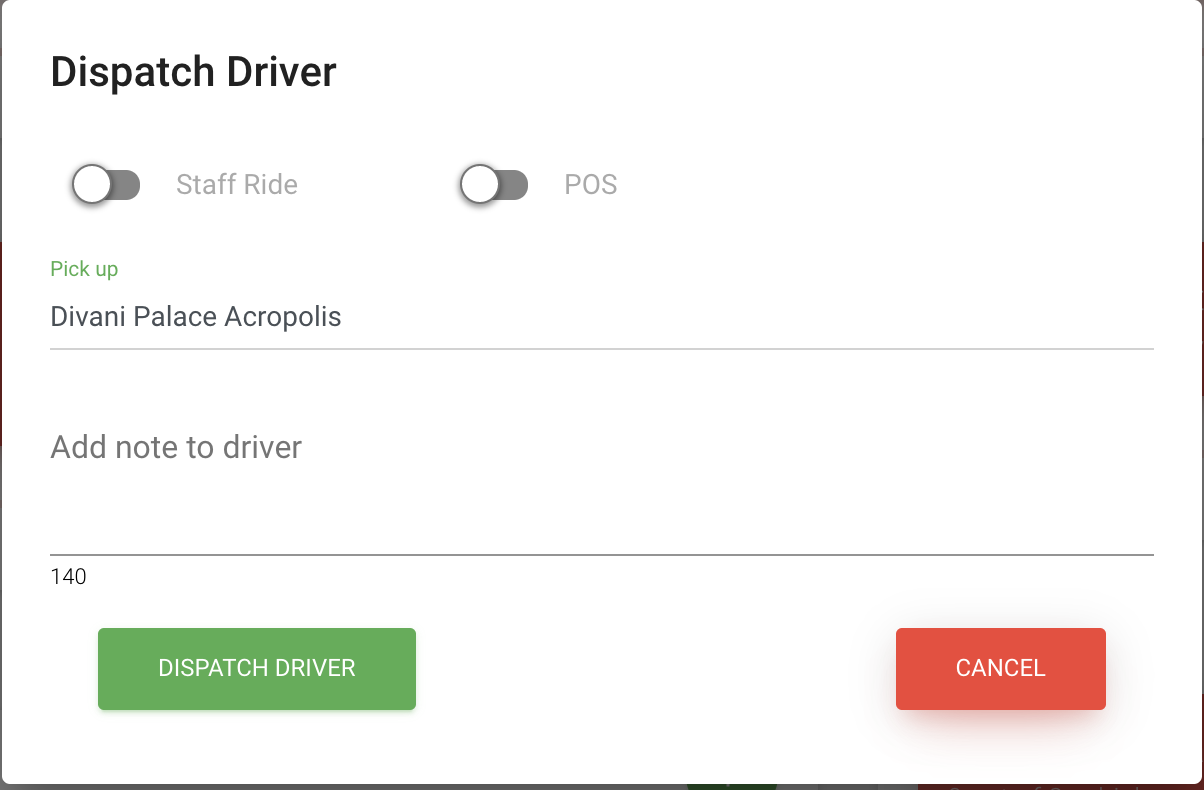
\includegraphics[scale=0.14]{images/my_projects/input/input-location-popup-new.png} }}%
	\qquad
	\subfloat[New Version-Input Display]{{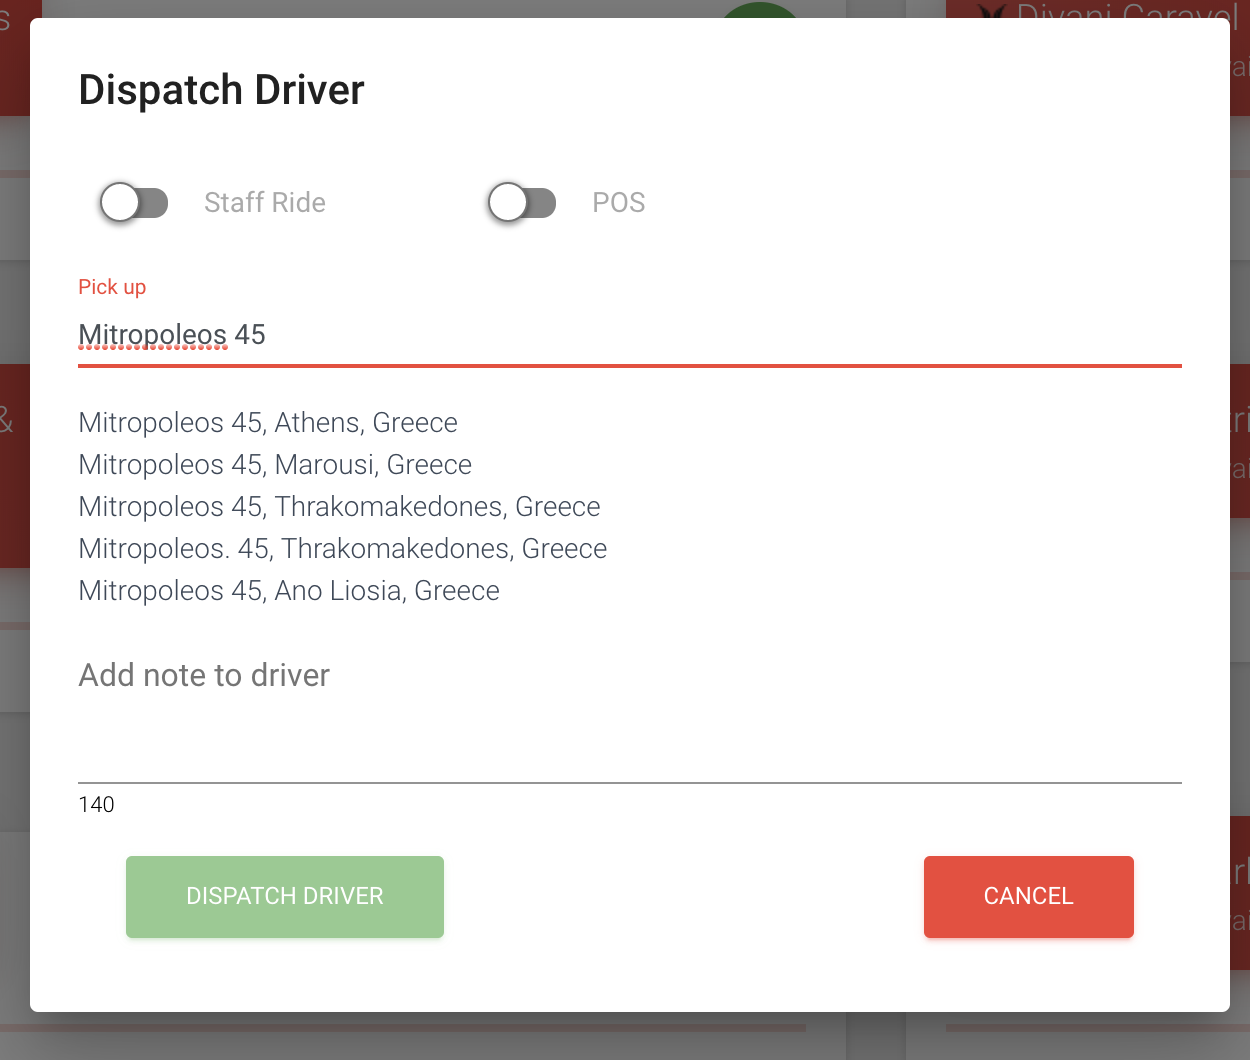
\includegraphics[scale=0.14]{images/my_projects/input/input-location-popup-input-new.png} }}%
	\caption{
		New Request Taxi Pop-up that includes an input for different pick-up location
	}
	\label{fig:example}
\end{figure}

As regards the project's technical details, there were added 529 lines of code, while 230 were deleted. The changed files were 15 in total and all of them have the extension either .jsx or .js, meaning that JavaScript and JSX code was written. More specifically, I created two new components named PlaceInput and DispatchDriverModel. The first one was for input creation and the other for abstracting the modal from the Dispatch component. Dispatch component used to contain all the information in Dispatch Tab shown both in 4.7 (A) and 4.8 (A). The library used for matching every possible location is "react-places-autocomplete".

\subsection{Best Practices \& Main Tools/Methods Used}

To complete this project, a variety of tools and practices gained from the Management Science and Technology Department were used. More specifically, the knowledge of selecting reliable libraries is learned in Trusted and Secure Software Development of the 6th semester. Moreover, the GitHub usage required for the project was given from the 6th semester's course in Software Engineering in Practice. Finally, the Internet \& Cloud Application Development course of the 7th semester provided the knowledge of how to create an auto-complete input form. \par

\subsection{Total Hours spend on the Project}

This project required restructuring components and new libraries to be added. It was a great change to how the dispatch of a taxi occurs and for this reason, it had to be tested in detail. The total hours spend on the project were about to 21, that match to 3 working days. \par

\subsection{Delays on Initial Schedule}

This project started on the 11th and completed on the 13th of June. Finally, my PR on GitHub about this feature was merged on June 14th and some days later it was also online on BeatHotel Agent Dashboard. \par

\begin{figure}[H]
	\begin{center}
		
\includegraphics[scale=0.85]{images/my_projects/input/input-location-PR.png}
	\end{center}
	\caption{Approved Pull Request}
\end{figure}

\subsection{Problems occurred} 

During the project's implementation, there were no serious problems occurred. The only issue was that since the pickup location was different, this information had to be displayed in some way to the agents. This was solved by adding a hovering in each ongoing ride that reveals its pick-up location. \par

\subsection{Estimation of Project's impact on the company}

The results of this specific project are important for Beat's Agents, Travel Agencies and Hotels. This feature gives to all of them, the opportunity of choosing a different pick-up location, and thus to use the service, whenever they need a taxi even if their location is not predetermined. This project was created mostly to cover travel agents needs. Travel Agencies are mainly requesting a taxi for their customer's transportation, who are in different pick-up locations every time. \par